\documentclass{article}
\usepackage{ctex}
\usepackage{makecell}
\usepackage{graphicx}
\usepackage{geometry}
\usepackage{multirow}
\usepackage{multicol}
\usepackage{fancyhdr}
\usepackage{longtable}
\usepackage{color}
\usepackage{float}
\usepackage{listings}
\usepackage{xcolor}
\usepackage{hyperref}
\usepackage{footnote}
\usepackage{paralist}
\usepackage{amsmath}
\usepackage{subcaption}

\newcommand{\tabitem}{~~\llap{\textbullet}~~}
\renewcommand{\labelitemii}{\textbullet}
\renewcommand{\labelitemiii}{\textbullet}

\let\itemize\compactitem
\let\enditemize\endcompactitem
\let\enumerate\compactenum
\let\endenumerate\endcompactenum
\let\description\compactdesc
\let\enddescription\endcompactdesc

\geometry{a4paper,left=25mm,right=20mm,top=25mm,bottom=25mm}

\title{数字图像处理实验五}
\author{09021227~金桥}
\date{\today}

\lstset{
    numbers=left,
    keywordstyle= \color{ blue!70},
    commentstyle= \color{red!50!green!50!blue!50},
    rulesepcolor= \color{ red!20!green!20!blue!20} ,
    % escapeinside=``,
    numberstyle=\tt,
    numbersep=0em,
    xleftmargin=2em,
    breaklines,
    aboveskip=1em,
    framexleftmargin=2em,
    frame=shadowbox,
    basicstyle=\tt,
    language=C++
}

\begin{document}

\maketitle

\section{实验目标}

\begin{enumerate}
    \item 课本410页图9.11,对指纹图分别进行(d)(e)(f)三步操作。最终结果图还是有断开,思考如何把断开处连接。
    \item 对指纹图分别进行Global Thresholding操作和Otsu's Thresholding操作,并对性能进行分析。
    \item 使用Canny算子检测边界,可调用函数,分析每一步操作作用,思考为什么会比Sobel方法更好。
\end{enumerate}

\section{过程与方法}

\subsection{膨胀与腐蚀}

膨胀与腐蚀参照课本提供算法,结构元素均为$3\times 3$大小的矩阵。

\subsection{阈值}

\subsubsection{Global Thresholding}

Global Thresholding算法如下:
\begin{itemize}
    \item 为全局阈值$T$选择一个初始的估计值。
    \item 使用初始值$T$进行阈值分割,此时图像分为两组像素:
    \begin{itemize}
        \item 大于阈值的像素组$G_1$以及小于阈值的像素组$G_2$.
    \end{itemize}
    \item 分别计算属于$G_1, G_2$像素的平均灰度值$m_1, m_2$.
    \item 对$m_1, m_2$计算一个新的阈值$T=\frac{m_1+m_2}{2}$.
    \item 重复之前的步骤,直到旧阈值与新阈值的差小于预设的值$\Delta$为止。这里设置$\Delta = 1$.
\end{itemize}

\subsubsection{Otsu's Thresholding}

Otsu's Thresholding算法如下:
\begin{itemize}
    \item 计算所有灰度的概率分布,设灰度为$i$的概率为$P_i$.
    \item 计算累计和$S(k)=\sum_{i=0}^kP_i$.
    \item 计算累计均值$m(k)=\sum_{i=0}^kiP_i$.
    \item 计算全局灰度均值$m_G$.
    \item 计算类间方差$\sigma_B^2(k)$,公式如下:$$\sigma_B^2(k)=\frac{(m_GS(k)-m(k))^2}{S(k)(1-S(k))}$$.
    \item Otsu阈值$k^*$为使得类间方差最大的$k$,即:$$k^*=\arg \max \sigma_B^2(k)$$
\end{itemize}

\subsubsection{Canny算子}

采用OpenCV的\texttt{cv::Canny}函数。

\section{结果与分析}

\subsection{膨胀与腐蚀}

\begin{figure}[htbp]
    \centering
    \begin{subfigure}{.22\textwidth}
        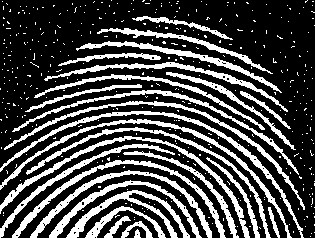
\includegraphics[width=\linewidth]{img/Fig0911(a)(noisy-fingerprint).jpg}
    \end{subfigure}
    \begin{subfigure}{.22\textwidth}
        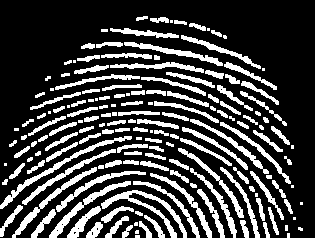
\includegraphics[width=\linewidth]{img/job1-d.png}
    \end{subfigure}
    \begin{subfigure}{.22\textwidth}
        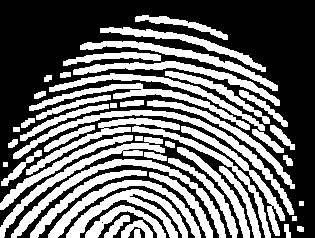
\includegraphics[width=\linewidth]{img/job1-e.png}
    \end{subfigure}
    \begin{subfigure}{.22\textwidth}
        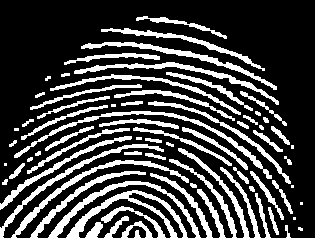
\includegraphics[width=\linewidth]{img/job1-f.png}
    \end{subfigure}
    \caption{课本410页图9.11,对指纹图分别进行(d)(e)(f)三步操作。最左侧为原图,右侧依次是(d)(e)(f).}
\end{figure}

\begin{figure}[htbp]
    \centering
    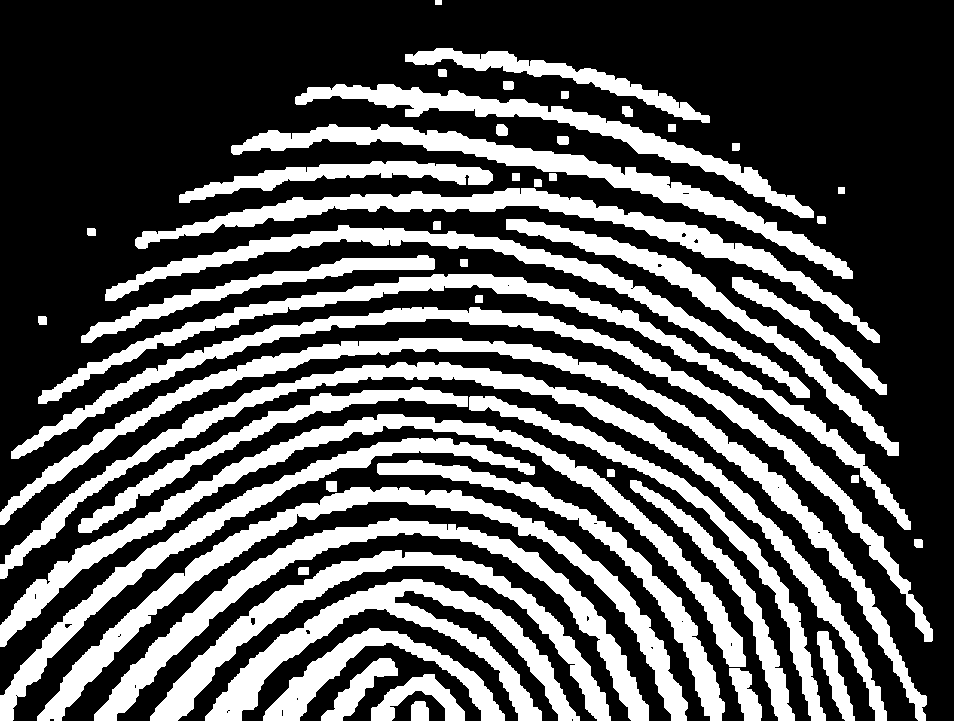
\includegraphics[width=0.3\linewidth]{img/connect.png}
    \caption{调大图像后应用多次膨胀与腐蚀的效果。指纹基本没有断开,但是也造成了噪声的保留。}
\end{figure}

通过调大图像或调小结构元,可以控制膨胀与腐蚀的力度,从而达到更精确的控制,使得指纹不会有断开的地方。但与此同时会造成一些噪点的保留。

\subsection{阈值处理}

Global Thresholding的时间复杂度为$O(KNM)$, $k$为迭代次数,$N, M$为图像宽度与高度。

Otsu's Thresholding的时间复杂度为$O(NM)$, $N, M$为图像宽度与高度。


\begin{figure}[htbp]
    \centering
    \begin{subfigure}{.32\textwidth}
        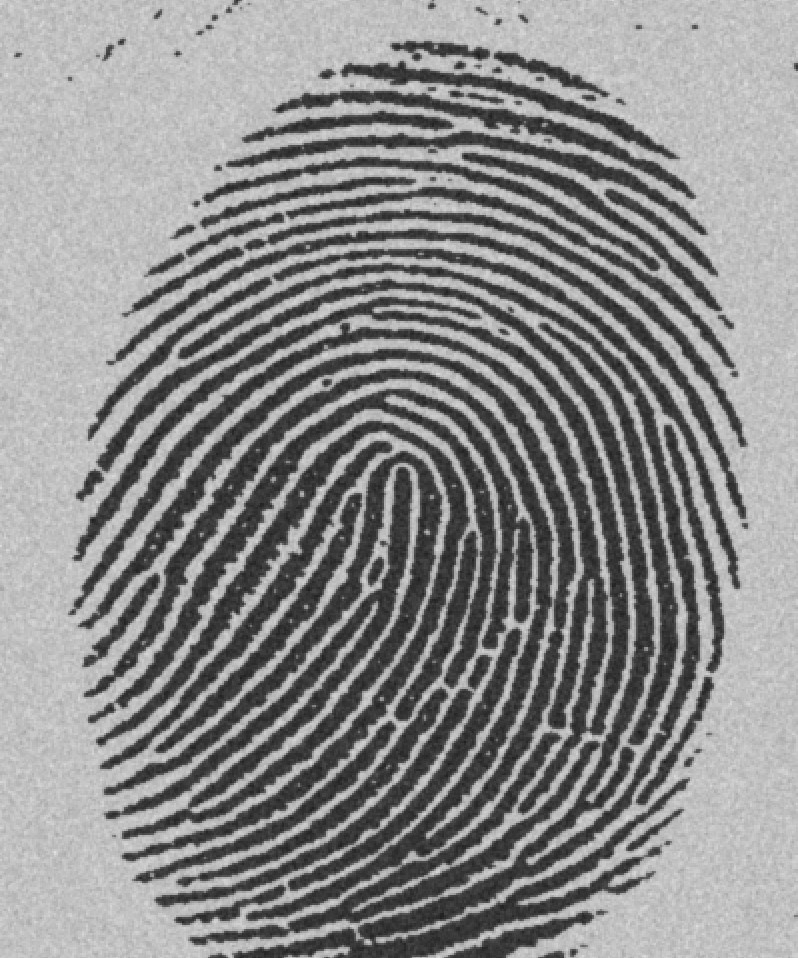
\includegraphics[width=\linewidth]{img/Fig1038(a)(noisy_fingerprint).jpg}
    \end{subfigure}
    \begin{subfigure}{.32\textwidth}
        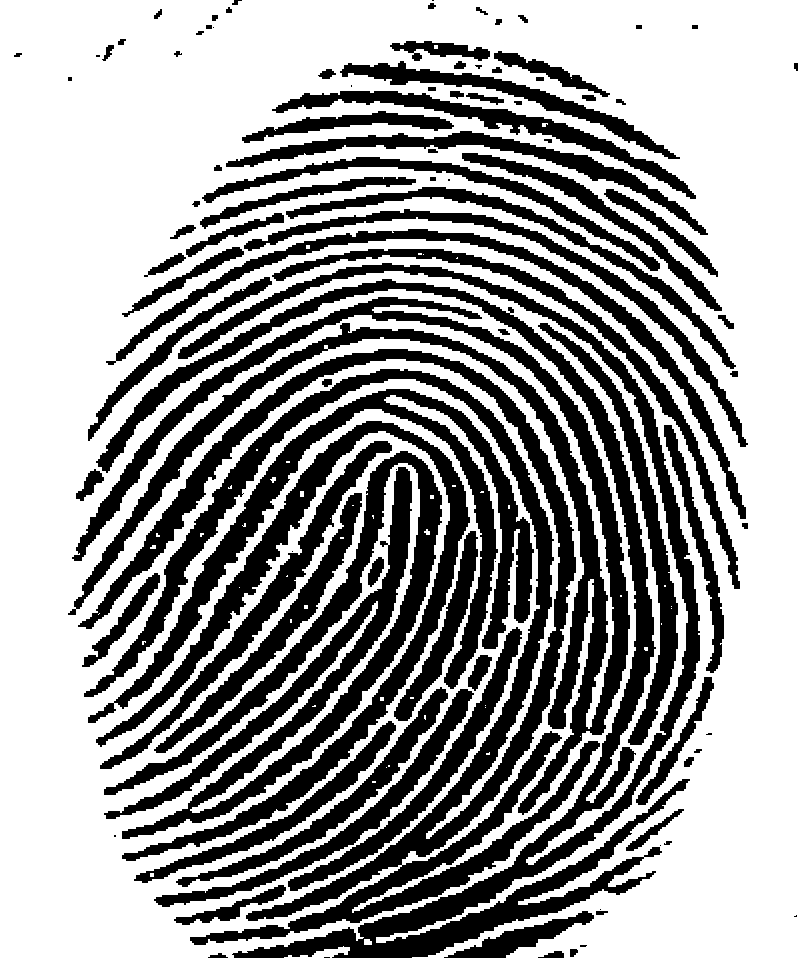
\includegraphics[width=\linewidth]{img/global-threshold.png}
    \end{subfigure}
    \begin{subfigure}{.32\textwidth}
        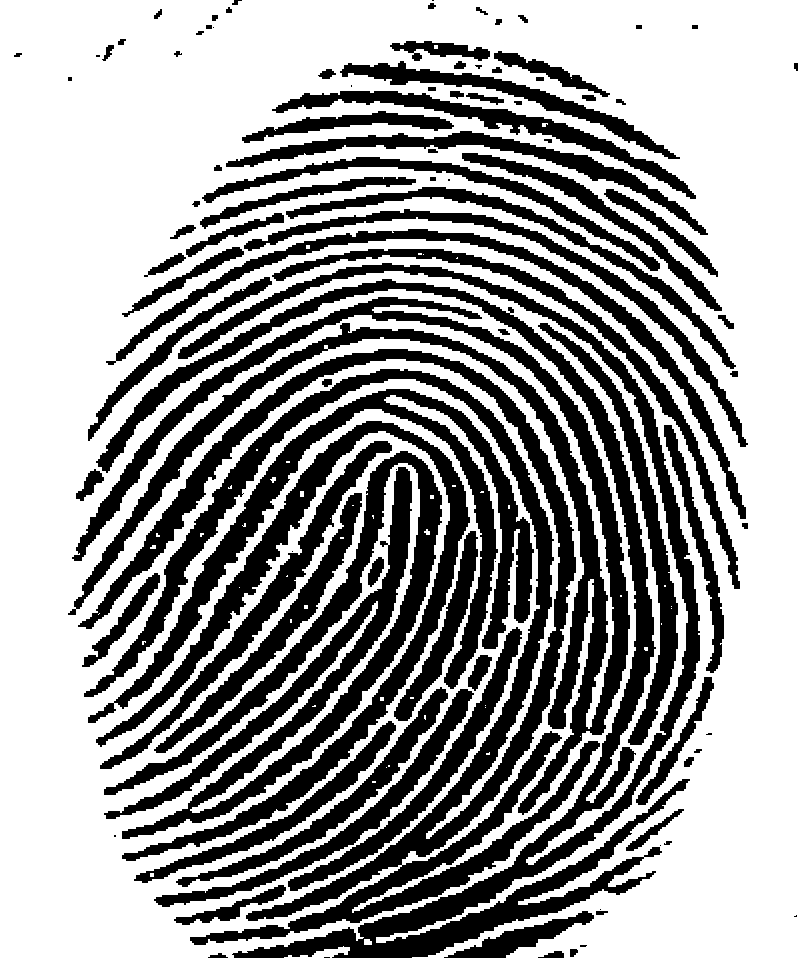
\includegraphics[width=\linewidth]{img/otsu-threshold.png}
    \end{subfigure}
    \caption{对指纹图分别进行Global Thresholding操作和Otsu's Thresholding操作。从左到右分别是原图,采用Global Thresholding处理的图像与采用Otsu's Thresholding处理的图像。由于图像本身的性质,所以这两种方式处理的效果基本一致。但实际上两幅图的直方图存在细微的差别。}
\end{figure}

\subsection{检测边界}

\begin{figure}[htbp]
    \centering
    \begin{subfigure}{.4\textwidth}
        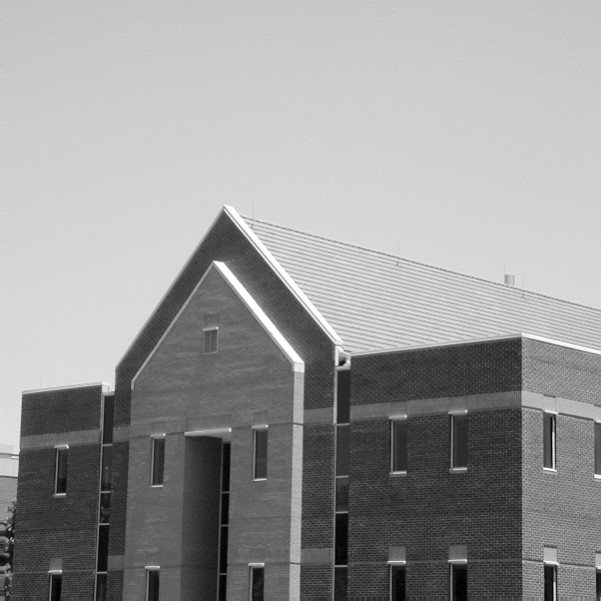
\includegraphics[width=\linewidth]{img/Fig1006(a)(building).jpg}
    \end{subfigure}
    \begin{subfigure}{.4\textwidth}
        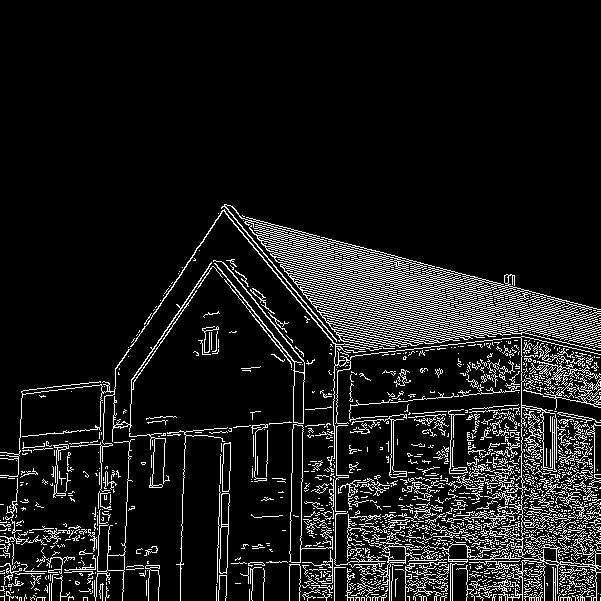
\includegraphics[width=\linewidth]{img/canny.png}
    \end{subfigure}
    \caption{采用OpenCV的\texttt{cv::Canny}进行边缘检测。左侧为原图,右侧为处理后的图像。}
\end{figure}


Canny算子检测边界的主要步骤与作用如下:

\begin{itemize}
    \item 去噪。噪声会影响边缘检测的准确性,因此首先要将噪声过滤掉。
    \item 计算梯度的幅度与方向。
    \item 非极大值抑制,即适当的让边缘变瘦。
    \item 确定边缘。使用双阈值算法确定最终的边缘信息。
\end{itemize}

相较于Sobel方法,Canny的优势在于:它能够尽可能多地标识出图像中的实际边缘,且标识出的边缘与实际图像中的实际边缘更接近。


\end{document}
